\begin{frame}{The fraction of \Y2S originating from \chib decays}
\setlength{\unitlength}{1mm}

\begin{center}
\textcolor{blue}{\sqs=7\tev}, \textcolor{red}{\sqs=8\tev}

\begin{picture}(100,40)
      %
    \put(0,0){
      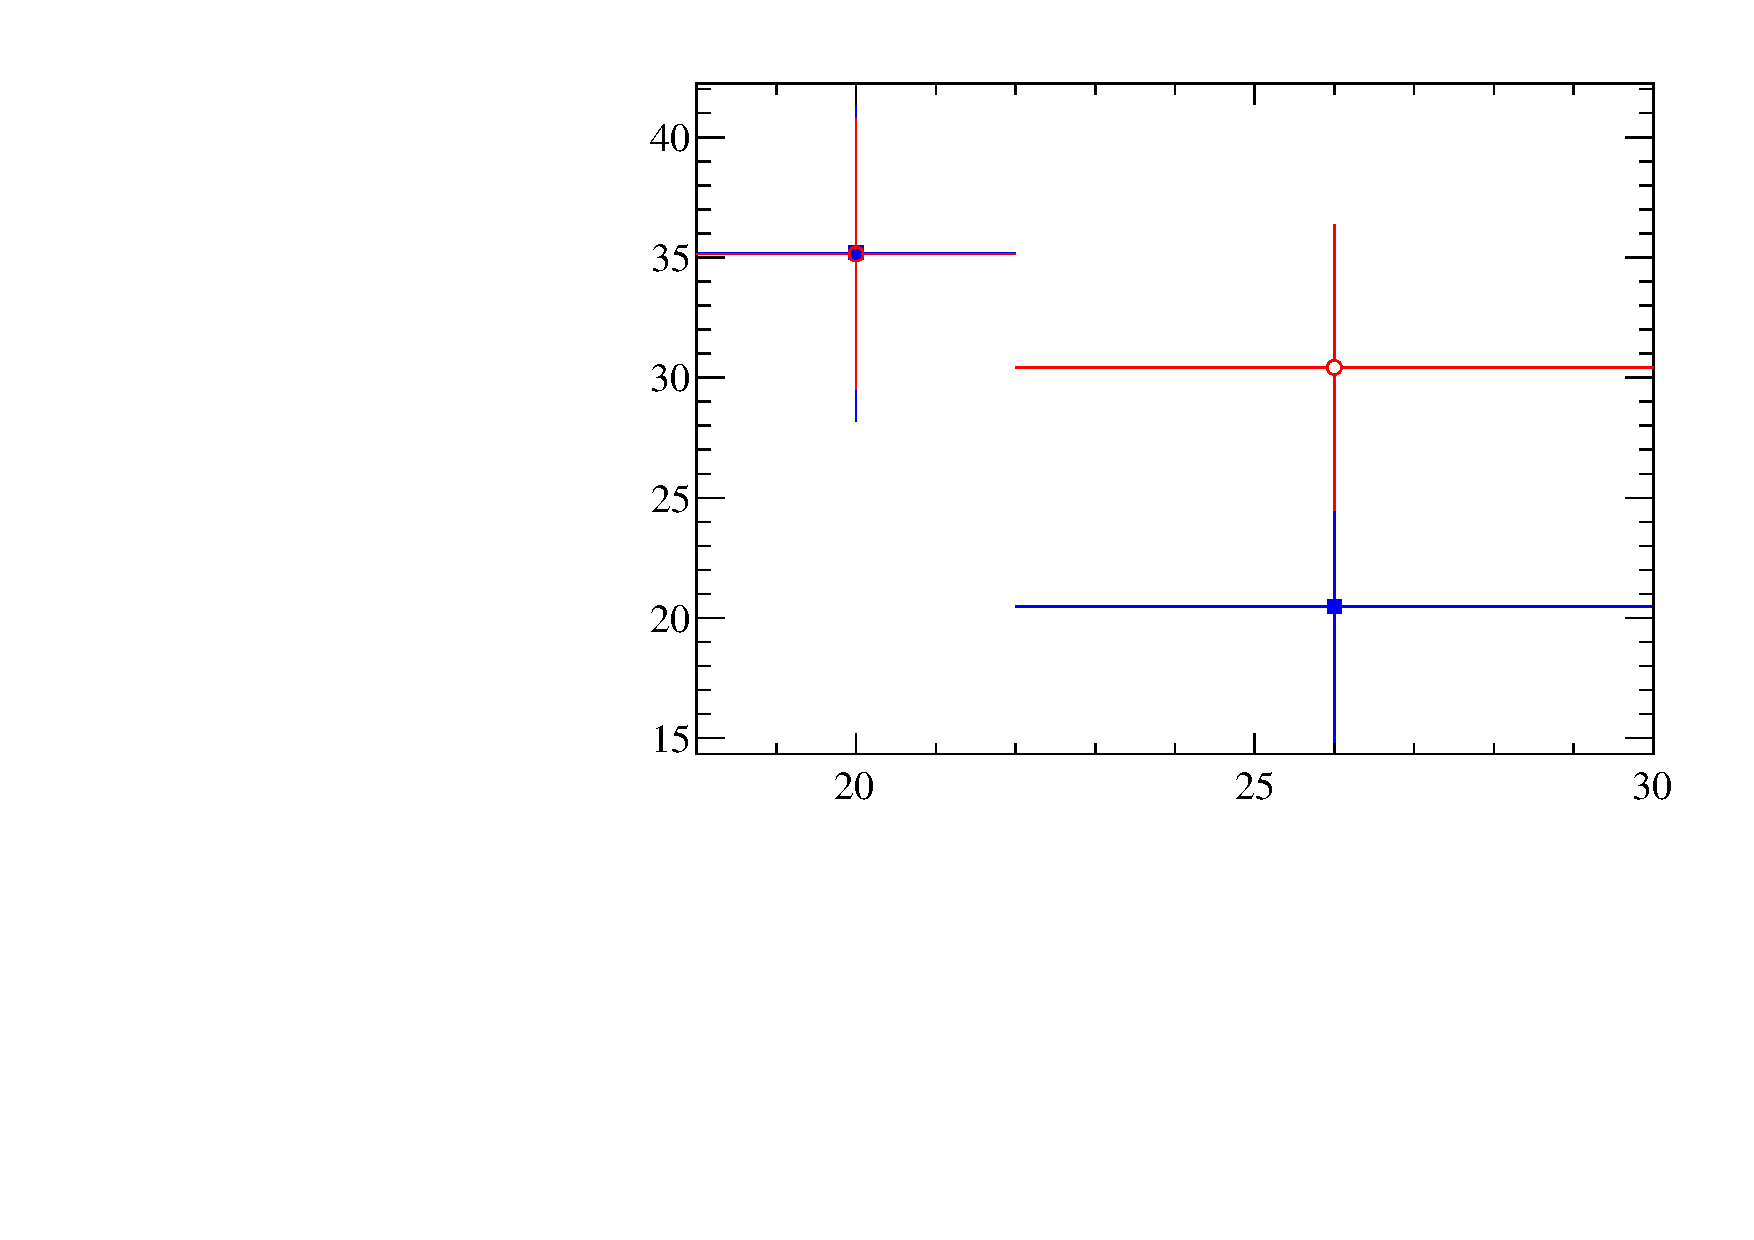
\includegraphics[width=50mm, height=40mm]{frac-2s/cb2_frac_2s}
    }
    \put(50,0){
      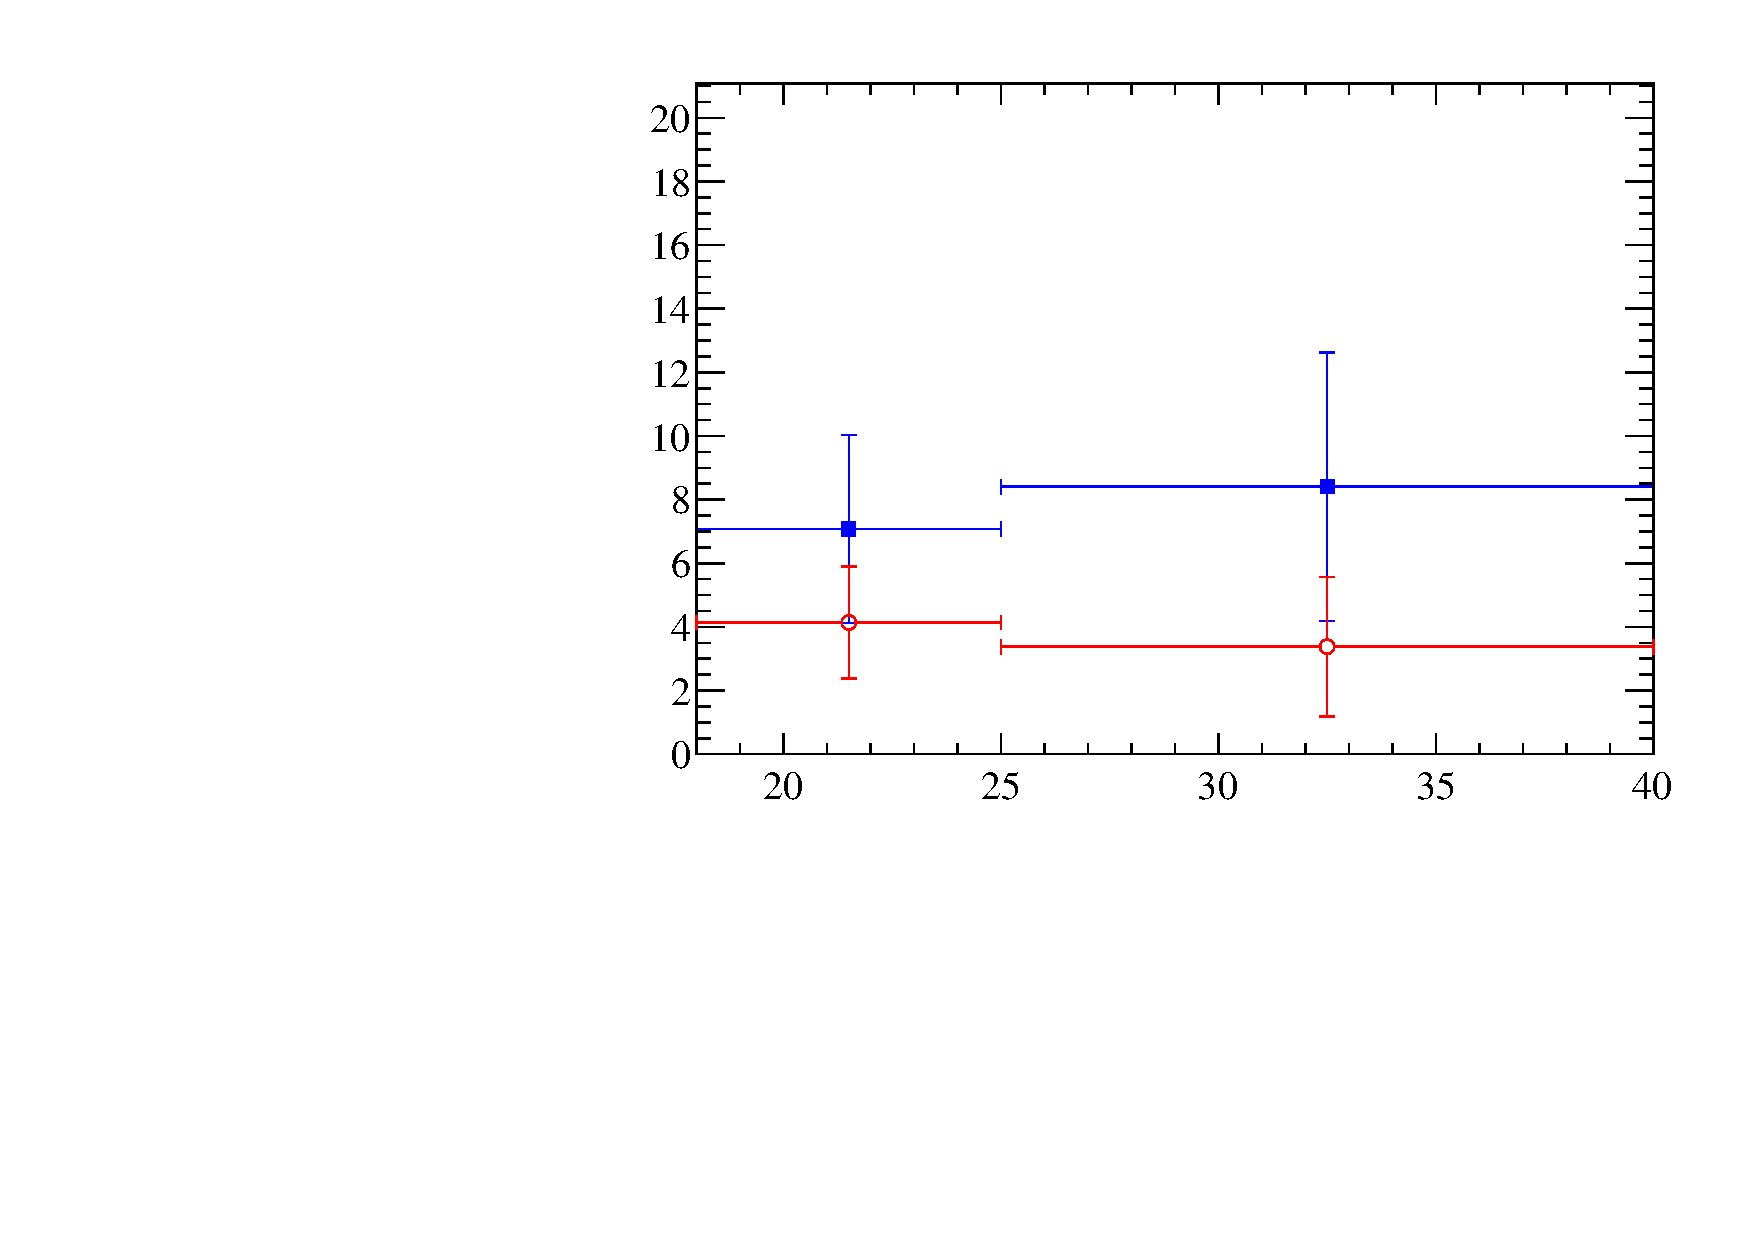
\includegraphics[width=50mm, height=40mm]{frac-2s/cb3_frac_2s}
    }    
    
   \put(2,12){\begin{sideways}Fraction (\%)\end{sideways}}
   \put(12,0){$p_T(\Y2S) \left[\gevcc\right]$}
   \put(10,35){\tiny $\chi_b(2P) \to \Y2S \gamma$}

   \put(52,12){\begin{sideways}Fraction (\%)\end{sideways}}
   \put(62,0){$p_T(\Y2S) \left[\gevcc\right]$}
   \put(60,35){\tiny $\chi_b(3P) \to \Y2S \gamma$}
  \end{picture}
\end{center}
\end{frame}